%\documentclass{article}
%\usepackage{graphicx,subfigure}
%\usepackage{caption,rotating}
%\begin{document}

\begin{figure}[p]
\centering
 \subfigure[Plate (i) Sheep 3437 Wrinkled]{
    \label{fig:trial1he(i)}
    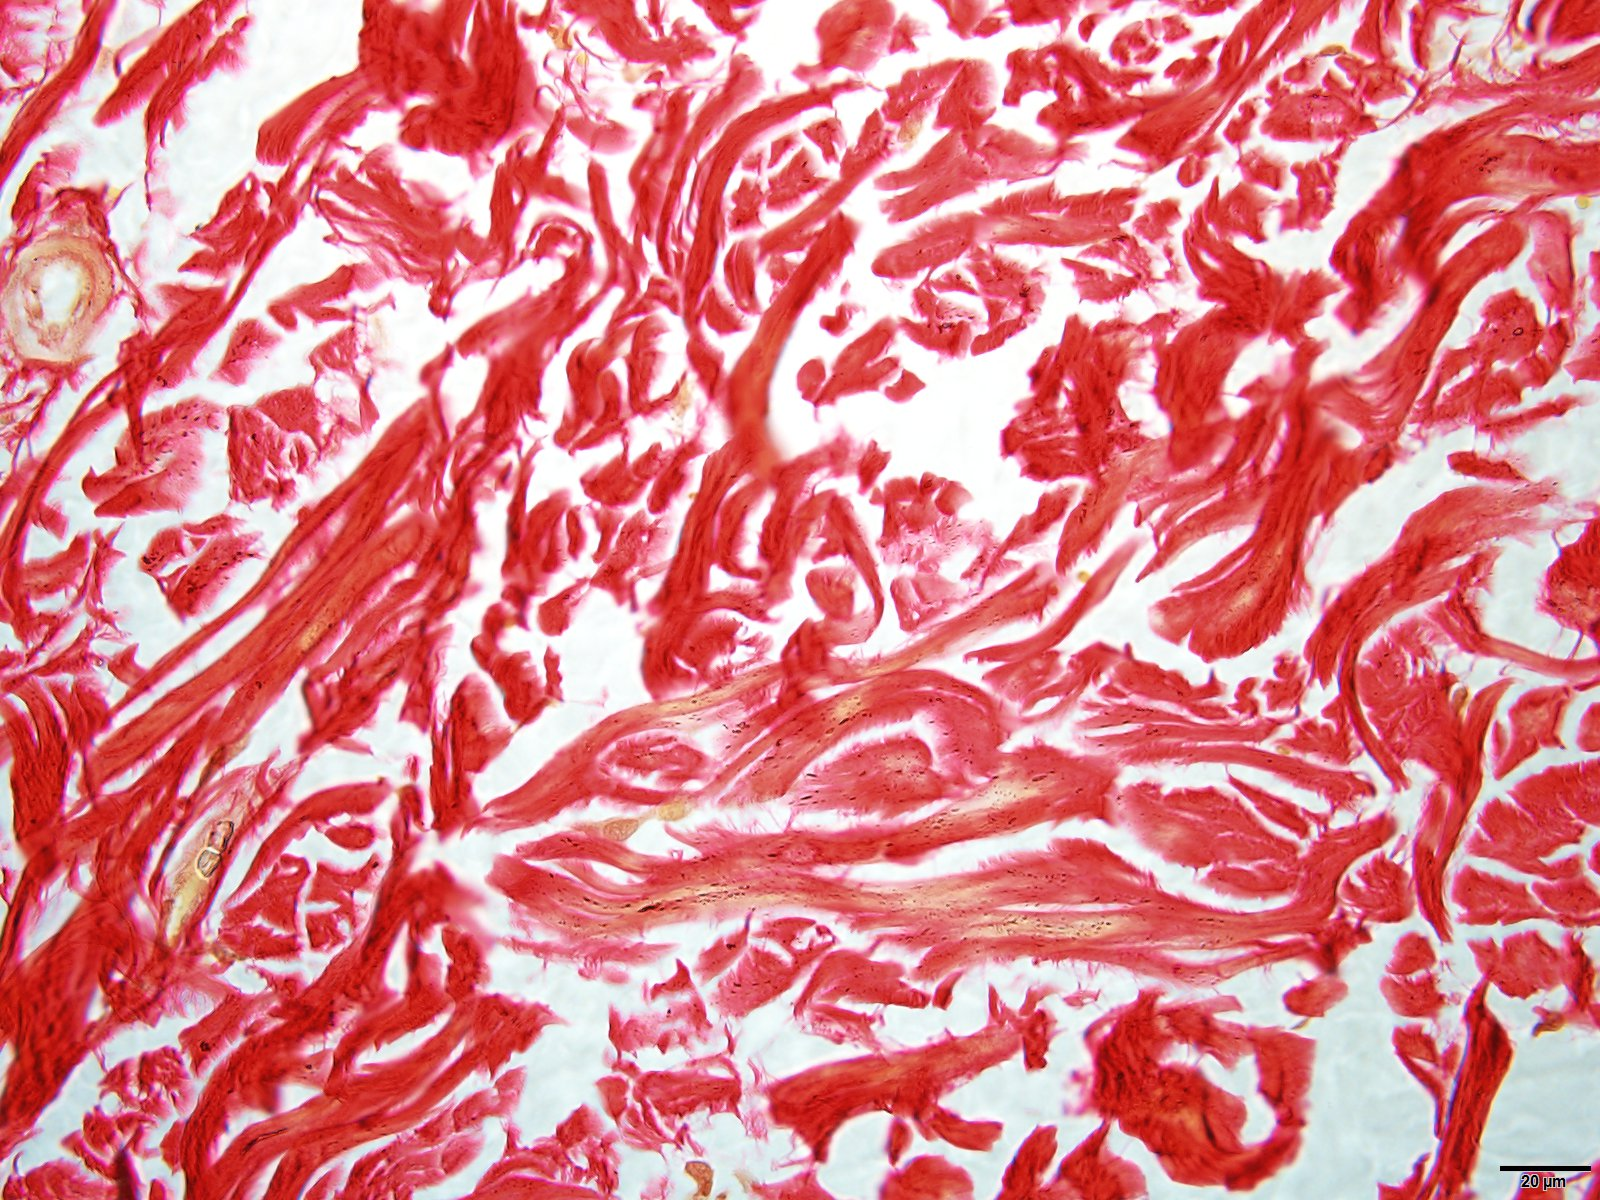
\includegraphics[scale=0.20]{3437_on_wrinkle_1.jpg}
% 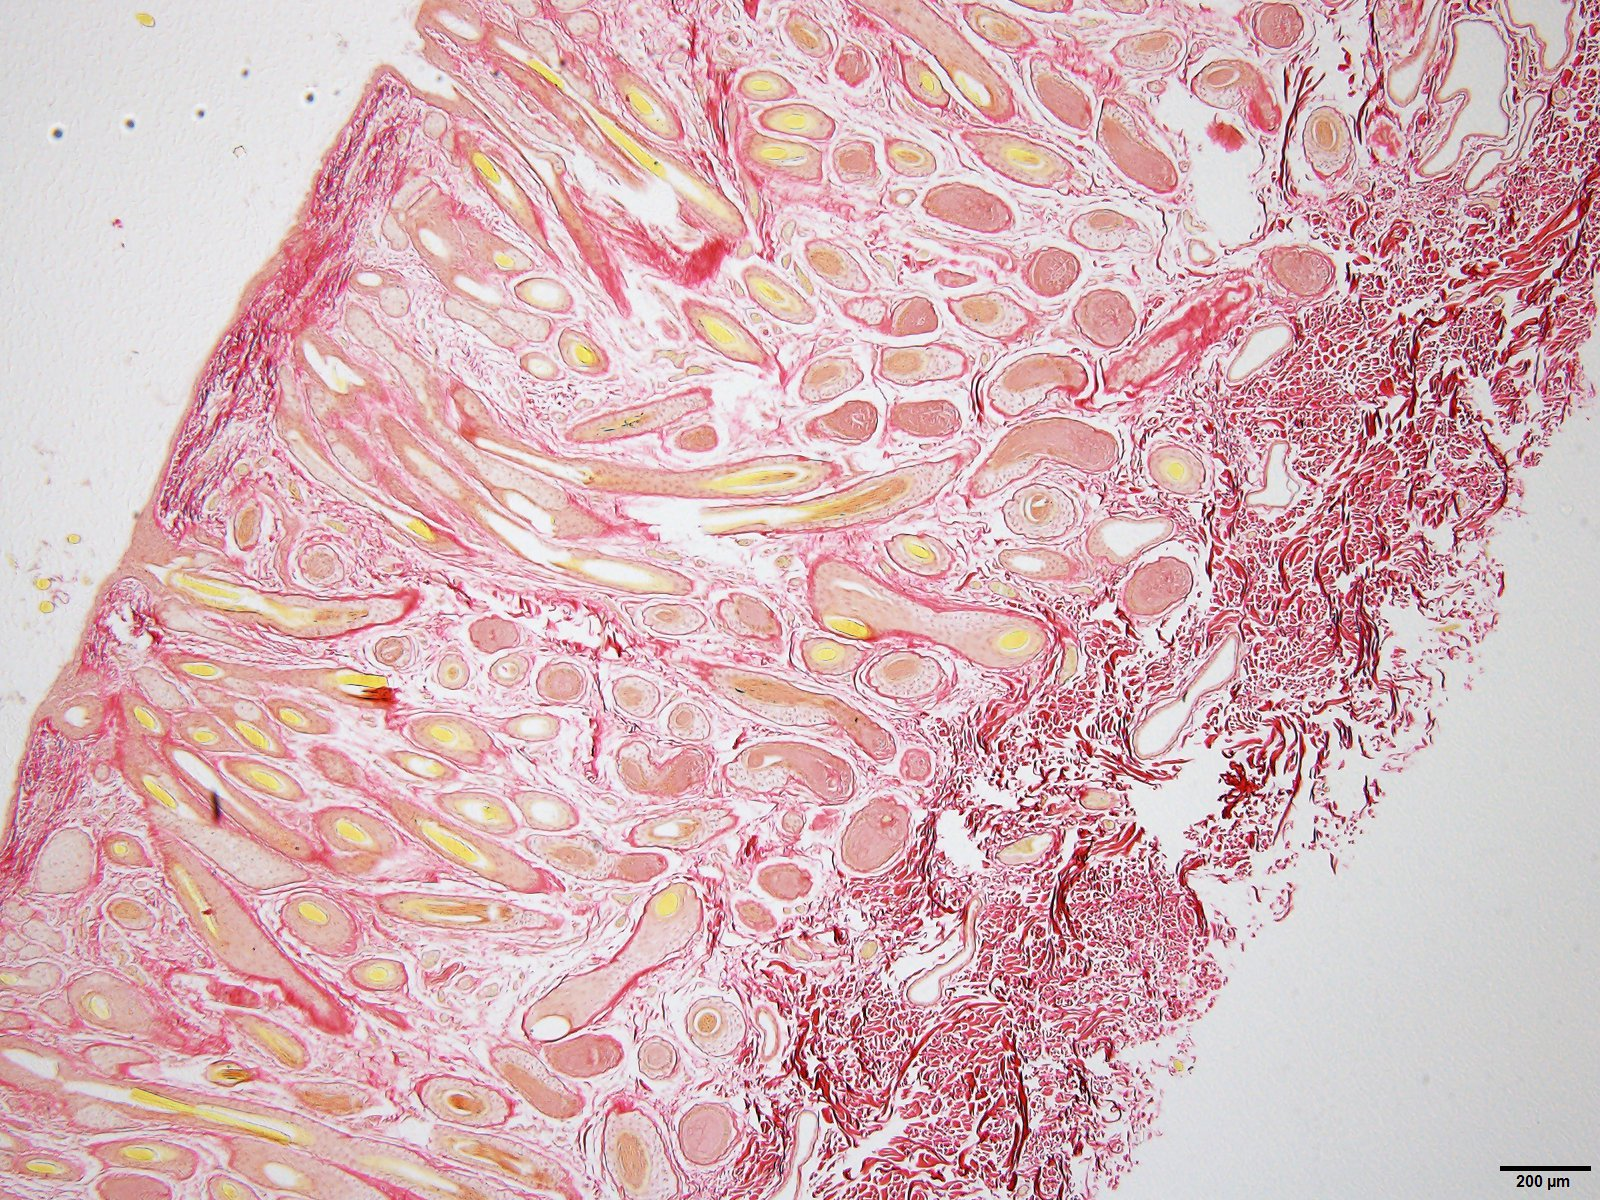
\includegraphics[width=1.0\textwidth]{w479-2-rigid.jpg}
  }
 \subfigure[Plate (ii) Sheep 3457 Wrinkle-free]{
    \label{fig:trial1he(ii)}
    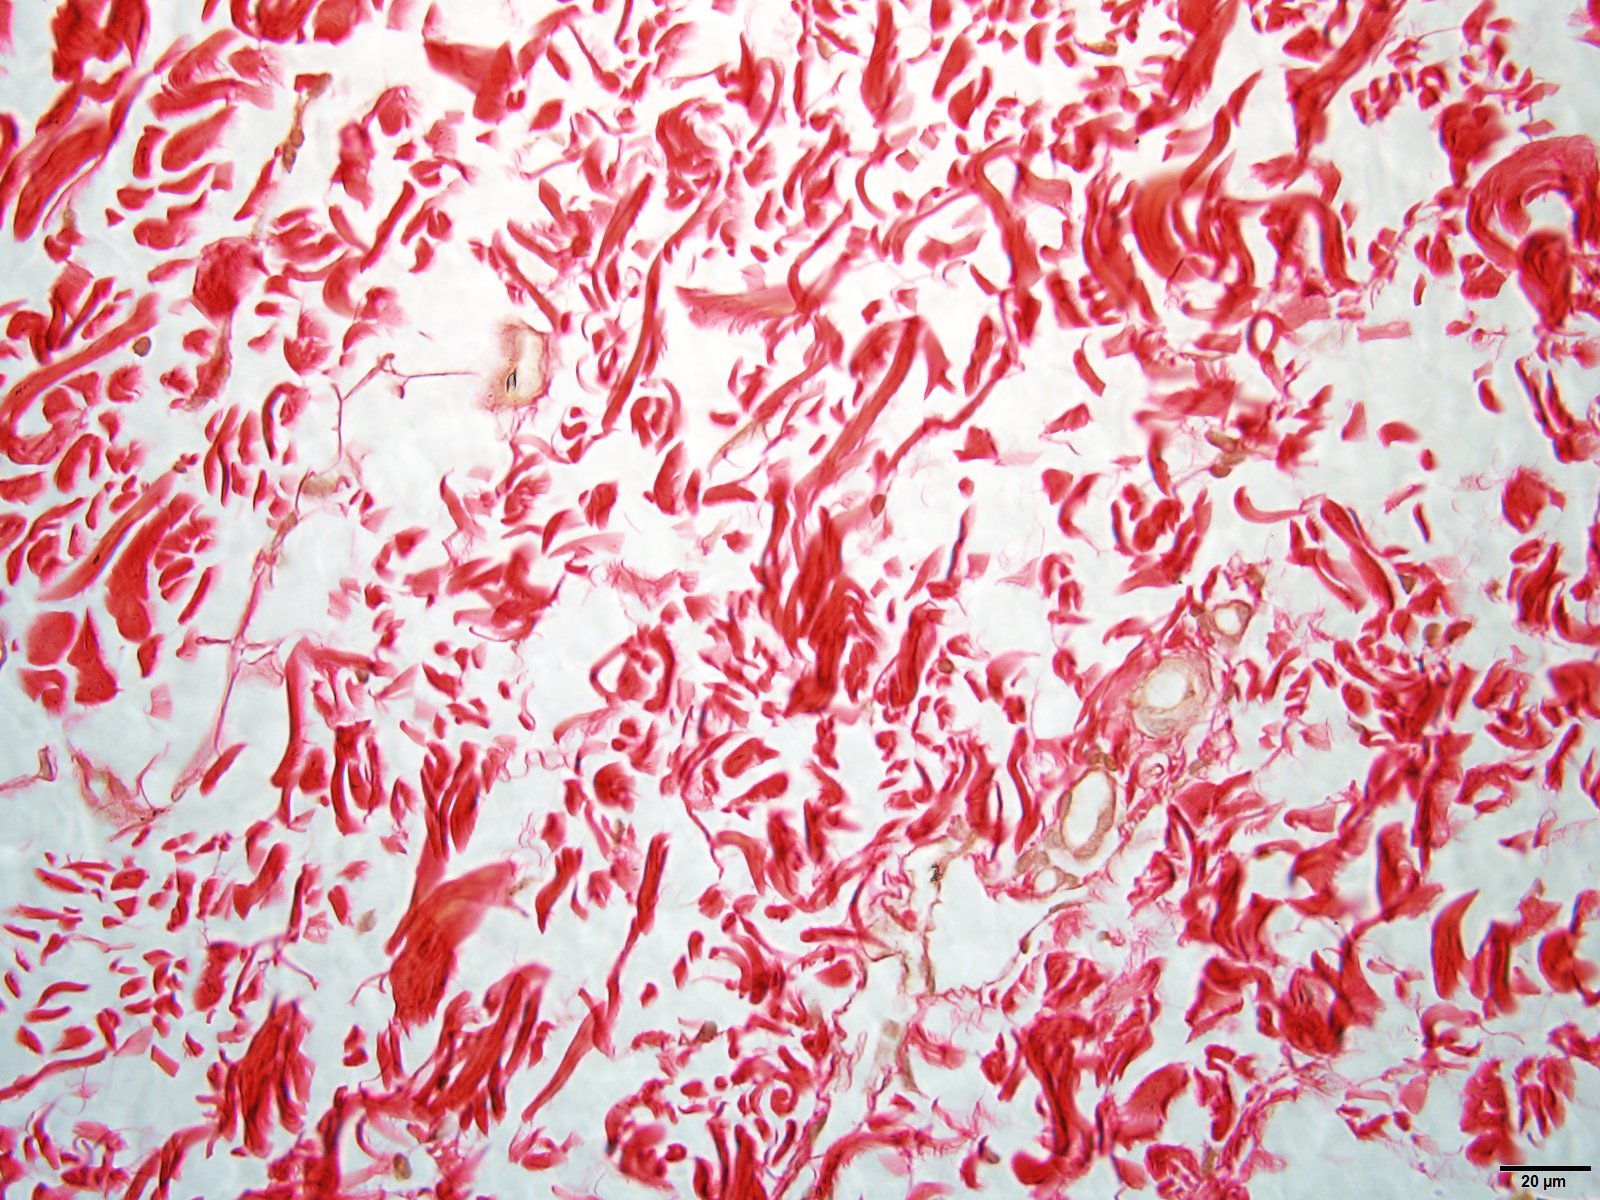
\includegraphics[scale=0.20]{3457_smooth_3.jpg}
  }
  \caption{Fields chosen at random from within Layer 3 (subpapillary dermis) stained with PSR and viewed with a 40x objective.}
\vfill
  \label{fig:psr40x}
\end{figure}

%\end{document}

